\begin{figure}
	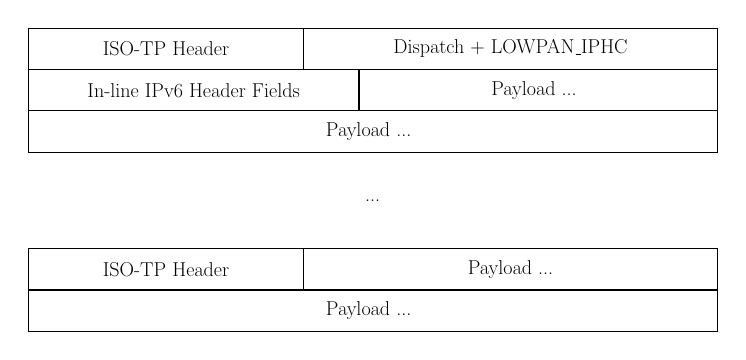
\begin{tikzpicture}[scale=0.35,  every node/.style={scale=0.35},
		region/.style={
			minimum height=1.5cm,
			align=left,
			draw,
			font=\huge}]

		\node (isotp) [region, anchor=west, minimum width=10cm] {ISO-TP Header};
		\node (iphc) [region, right of = isotp, xshift=11.5cm, minimum width=15cm] {Dispatch + LOWPAN\_IPHC};
		\node (inline) [region,anchor=west, yshift=-1.5cm, minimum width=12cm] {In-line IPv6 Header Fields};
		\node (payload) [region, right of=inline, xshift=11.5cm, minimum width=13cm] {Payload ... };
		\node (dayload2) [region,anchor=west, yshift=-3cm, minimum width=25cm] {Payload ... };

		\node at (12.5cm, -5.5cm) {\huge ...};

		\node (isotp2) [region, anchor=west, yshift=-8cm, minimum width=10cm] {ISO-TP Header};
		\node (iphc3) [region, right of = isotp2, xshift=11.5cm, minimum width=15cm] {Payload ...};
		\node (dayload4) [region,anchor=west, yshift=-9.5cm, minimum width=25cm] {Payload ... };
	\end{tikzpicture}
\end{figure}